\documentclass[10pt]{beamer}
\usepackage{beamerthemesplit, amsmath, graphicx, bbm, multicol, multirow}

\usetheme{Berkeley}

\DeclareMathOperator*{\argmax}{argmax}
\DeclareMathOperator*{\argmin}{argmin}
\renewcommand{\baselinestretch}{1.2}

\title{Calculating Potential Exposure at CCG}
\author{Adrian Dr\u{a}gulescu, John Scillieri, et al.}
\date{November 5, 2007}
\institute{Risk Management Group\\
Constellation Energy}


\begin{document}

\frame{\titlepage}

%% overview page
\frame{
  \frametitle{Overview}
  \tableofcontents
}

%% motivation
\section{Existing MPE technology}

% motivation
\frame
{
  \frametitle{Existing MPE technology}
\begin{itemize}
\item The current techology was developed in various stages since mid-2002
by RMG.  Over time, we expanded it based on various requests
from the Credit group and the Front Office. 

\item There were several attempts to standardize the runs and provide
  a GUI because the requirements kept ramping up.  

\item Calculating the MPE should be straightforward, easy, and (preferably) 
not require RMG involvement.  We are not there yet.  
\end{itemize}
}

\frame
{
  \frametitle{``Features'' of existing MPE technology}
\begin{itemize}
\item Developed in Matlab.  Licenses can sometimes be an issue. 
\item Matlab templates used were often an older version (London). 
\item Currently only runs interactively. 
\item Matlab runs on local PC so big portfolios cannot fit in memory. 
\item Have support for many deal types.
\item One run cannot be combined with an existing portfolio. 
\item Backtesting is done by request, not fully automated.
\item Running calculators in SecDB and importing positions in Matlab
  is slow. 
\item Long deals can take a long time to simulate.
\item The price simulation uses SecDB volatilities, price caps, do the
  prices make sense? 
\item Who did not have problems with a heat rate deal?  Is Haibin in
  today?  
\end{itemize}
}

\frame
{
  \frametitle{Current/Old price simulation model}
\begin{itemize}
\item One factor GBM with mean reversion to mimic SecDB (as in 2002). 
\item The volatilities used are the SecDB implied vols. Market quotes 
  are sparse.  Some power vol quotes were very high.  Other
  commodities were not marked, and had very low implied vols.   
\item Based on our initial experience with power, we added a 50$\%$ vol
  cut to the SecDB vols.  It was not a good idea for other commods. 
\item Mean reversion was set by commodity but the levels were too
  low.  This was always an issue, because prices
  would difuse to historically ridiculous levels after 3 years. 
\item We introduced price caps/floors to remedy this.   
\item We boldly simulate a 20 year deal when we have no fundamental
  reason to believe forward marks beyond 4th year out (at best). 
\end{itemize}
}

\frame
{
  \frametitle{Current/Old price simulation model}
\begin{itemize}
\item Correlations were estimated historically. 
\item Introduced heat-rate caps/floors too. 
\item Problem with ancillary curves, or curves that move infrequently,
  see NOX, etc. 
\end{itemize}

{\Large If we have so many issues are all our MPE numbers wrong?  NO!} 

\vspace{\baselineskip}
{\Large But if you know of so many issues why don't you fix it? We are!} 
}

%%%%%%%%%%%%%%%%%%%%%%%%%%%%%%%%%%%%%%%%%%%%%%%%%%%%%%%%%%%%%%%%%%%%%
%% Goals section
%%%%%%%%%%%%%%%%%%%%%%%%%%%%%%%%%%%%%%%%%%%%%%%%%%%%%%%%%%%%%%%%%%%%%
\section{Our goals (by the end of 2007)}
\frame
{
  \frametitle{Goals for the new MPE}
\begin{itemize}
\item Ability to calculate exposure by counterparty, by portfolio, by
  deal. 
\item Have realistic price simulations based on history.    
\item Have daily reporting on future exposures and changes. 
\item Have ability to report on historical MPE by counterparty.
\item Periodic (automatic) backtesting of predetermined deals. 
\item Improved interaction with SecDB for position gathering. 
\item No more bargaining with the Origination on the ``vol cut''.  If
  Origination requests a different exposure, the reason will be
  entered in a database. 
\end{itemize}
}

%--------------------------------------------------------------------
\frame
{
  \frametitle{Challenges for the New/Current MPE}
\begin{itemize}
\item Simulation of a few correlated time series is trivial. 
\item For our problem, major challenge is the scale of the data. 
\begin{itemize}
\item Around 700 distinct curves with various history
\item 24 to 60 contract month for each curve
\item Correlations among 30,000 curve/month must be kept
\end{itemize}
\item Positions with about 800 counterparties.  
\end{itemize}
}

%%%%%%%%%%%%%%%%%%%%%%%%%%%%%%%%%%%%%%%%%%%%%%%%
%% Implementation
%%%%%%%%%%%%%%%%%%%%%%%%%%%%%%%%%%%%%%%%%%%%%%%%

\section{New MPE Implementation}

\frame 
{
  \frametitle{Price simulation}
Understanding of the historical data is crucial in forward
simulation.  
\begin{enumerate}
\item Took a hierarchical view on the data and built a curve pedigree. 
There are parents and children curves.
\item Use PCA for dimension reduction.
\item Simulate correlated parents based on OU process assumption.
\item Simulated children based on simulated parents.
\end{enumerate}

Practically:
\begin{itemize}
\item Hand pick the parents (the representative/base curves).  
\item Natural Gas, Coal, Oil, International Coal.
\item Many other markets that are quasi independent.  
\item Electricity and its dependency on fuels.
\end{itemize}
}

\frame
{
  \frametitle{Example of the curve hierarchy} 
\begin{center}
  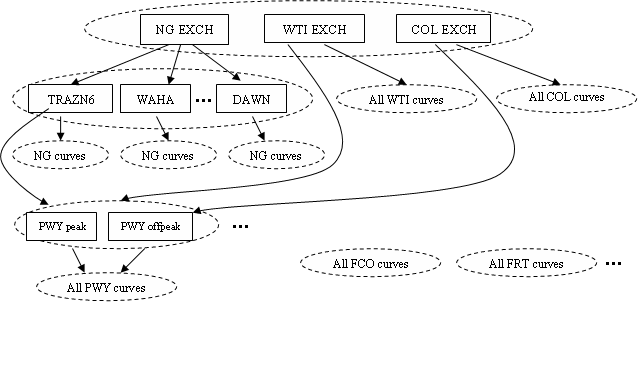
\includegraphics[height=2.5in]{figures/pedigree.png}
\end{center}
}

\frame 
{
  \frametitle{Implementation decisions}
We had to depart from the old simulation philosophy.
\begin{itemize}
\item We let the history speak.  More price history is better.  We
  want at least 3+ years.  But we need clean data. 
\item We simulate only up to 4 years out.  For contracts farther out,
  price changes are added on top of the current marks. 
\item This means that for a 10 year deal we're only going to show you
  the exposure for the next 4 years.  We're not that infatuated
  to believe we can predict price ranges beyond 4 years without a
  fundamental model.  
\item The good news is that groups of curves, markets can have
  different models.  So we can model the FRT \& FRC curves separately. 
\end{itemize}
}


\frame
{
  \frametitle{Implementation decisions}
\begin{itemize}
\item Only linear deal type will be supported.  No more heat rates,
  options, etc.  It is simply not worth pursuing full valuation at
  this stage.  And it will be a show stopper. 
\item Performance results:
\begin{itemize}
  \item 1000 simulations for all curves takes less then 2 hours. 
  \item Calculating the exposure for all counterparties is about 1
    hour. 
\end{itemize}
  \item The code was written in the Open Source statistical 
    programming language {\tt R}.  No licenses issue.  Ever. 
\end{itemize}
}

%%%%%%%%%%%%%%%%%%%%%%%%%%%%%%%%%%%%%%%%%%%%%%%%
%% Future work
%%%%%%%%%%%%%%%%%%%%%%%%%%%%%%%%%%%%%%%%%%%%%%%%

\section{Future Work (by the end of 2007)}

\frame
{
  \frametitle{Future steps}
\begin{itemize}
\item Continue testing the model and make it production ready. 
\item We were setback when trying to add more historical data.
  We're almost done with that. 
\item We've build some backtesting facilities.  Need to expand them. 
\item Integrate the R development with the Web interface. 
\item We have code ready to pull positions directly from calculators.
\item We have code ready to calculate a Credit VaR using the Credit Risk+
  method.  Need data from RAFT to publicize this daily.  
\end{itemize}
Only foreseeable risk is other assignments from Aram.  In Jan-08, you
should be able to use this new tool. John, Haibin, Jing and I will
support you and all further development. 

}

\section{Future Future Work (through 2008)}

\frame
{
  \frametitle{Future Future steps}
\begin{itemize}
\item Start adding full valuation capability (end of 2008).
\item Investigate alternative models.  Modeling volatility.  Add the
  ability to add a ``fundamental'' view (trend).
\item Other possible items. 
\end{itemize}
}






\end{document}
